

\subsection{Constant time approximation}

We introduce a technique to transform approximations algorithms
into constant time algorithms that approximate the size of the optimal solution. 
In our case, we expose the technique for the approximating of the size 
of a maximal matching in some graph.


\subsubsection{A constant time algorithm}

In this paper, we shall denote our graphs $G$ as a couple of set $(V,E)$, whose first
component enumerates all vertices and the second component gives all edges. Besides,
we shall use the symbol $n$ to denote the cardinality of $V$ and we shall consider 
that the $G$'s degree is bounded by $d$.

\begin{definition}
Let $G = (V,E)$ be a graph, a \emph{matching} $M$ in $G$ is a set of pairwise non-adjacent
edges; that is, no two edges share a common vertex. A \emph{maximal matching} is a matching $M$
of a graph $G$ with the property that if any edge not in $M$ is added to $M$, then it is no longer a matching.
\end{definition}

\begin{remark}
Do not mistake maximal matchings with \emph{maximum matchings}, which are matchings containing the largest possible number of edges.
\end{remark}

\tikzstyle{vertex}=[circle,fill=black!25,minimum size=20pt,inner sep=0pt]
\tikzstyle{selected vertex} = [vertex, fill=red!24]
\tikzstyle{edge} = [draw,thick,-]
\tikzstyle{weight} = [font=\small]
\tikzstyle{selected edge} = [draw,line width=5pt,-,red!50]


\begin{figure}[h]
\centering
\subfloat[A matching non maximal.]
{
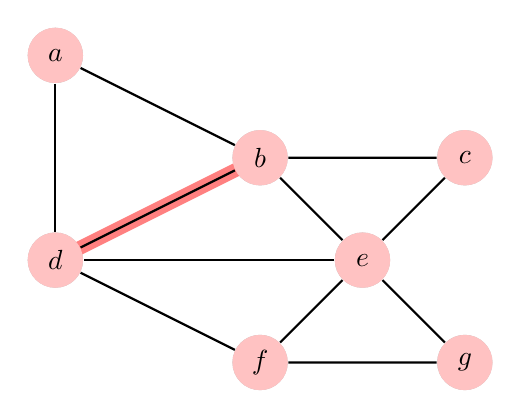
\begin{tikzpicture}[scale=1.3]
    \foreach \pos/\name in {{(0,2)/a}, {(2,1)/b}, {(4,1)/c},
                            {(0,0)/d}, {(3,0)/e}, {(2,-1)/f}, {(4,-1)/g}}
        \node[vertex] (\name) at \pos {$\name$};
	\path[selected edge] (d.center) -- (b.center);
%	\path[selected edge] (f.center) -- (e.center);
    \foreach \source/ \dest  in {b/a, c/b, d/a, d/b, e/b, e/c, e/d, f/d, f/e, g/e, g/f}
        \path[edge] (\source) -- (\dest);
    \foreach \vertex / \fr in {d/1,a/2,f/3,b/4,e/5,c/6,g/7}
        \path node[selected vertex] at (\vertex) {$\vertex$};
\end{tikzpicture}
}
\subfloat[A maximal matching non maximum.]
{
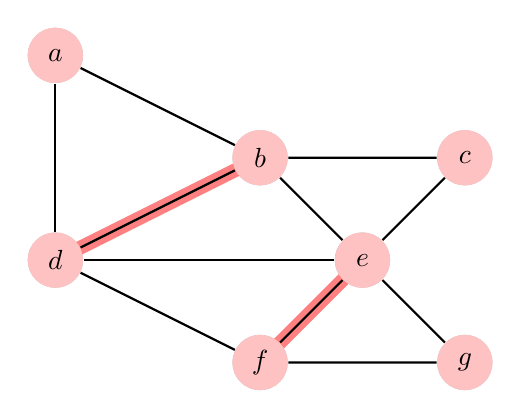
\begin{tikzpicture}[scale=1.3]
    \foreach \pos/\name in {{(0,2)/a}, {(2,1)/b}, {(4,1)/c},
                            {(0,0)/d}, {(3,0)/e}, {(2,-1)/f}, {(4,-1)/g}}
        \node[vertex] (\name) at \pos {$\name$};
	\path[selected edge] (d.center) -- (b.center);
	\path[selected edge] (f.center) -- (e.center);
    \foreach \source/ \dest  in {b/a, c/b, d/a, d/b, e/b, e/c, e/d, f/d, f/e, g/e, g/f}
        \path[edge] (\source) -- (\dest);
    \foreach \vertex / \fr in {d/1,a/2,f/3,b/4,e/5,c/6,g/7}
        \path node[selected vertex] at (\vertex) {$\vertex$};
\end{tikzpicture}
}\\
\subfloat[A maximum matching (maximal).]
{
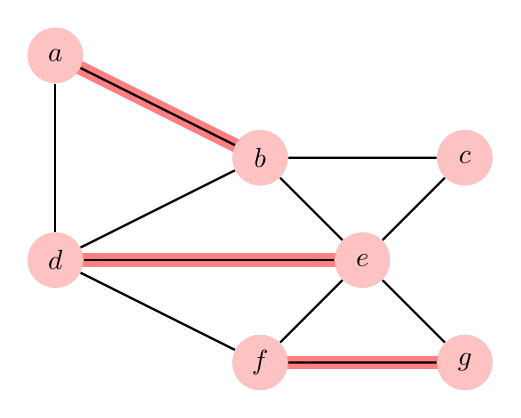
\begin{tikzpicture}[scale=1.3]
    \foreach \pos/\name in {{(0,2)/a}, {(2,1)/b}, {(4,1)/c},
                            {(0,0)/d}, {(3,0)/e}, {(2,-1)/f}, {(4,-1)/g}}
        \node[vertex] (\name) at \pos {$\name$};
	\path[selected edge] (a.center) -- (b.center);
	\path[selected edge] (d.center) -- (e.center);
	\path[selected edge] (f.center) -- (g.center);
    \foreach \source/ \dest  in {b/a, c/b, d/a, d/b, e/b, e/c, e/d, f/d, f/e, g/e, g/f}
        \path[edge] (\source) -- (\dest);
    \foreach \vertex / \fr in {d/1,a/2,f/3,b/4,e/5,c/6,g/7}
        \path node[selected vertex] at (\vertex) {$\vertex$};
\end{tikzpicture}
}
\caption{Matchings}
\end{figure}


\emph{Main algorithm} takes as input an oracle \emph{Magic test} whose job is to simulate the usual linear time greedy algorithm that we use to build a maximal matching, but in constant time. Thus, main algorithm will return in bounded time a good approximation of the size of a maximal matching $M$ of $G$.
%Computing the size of a maximal matching in a constant degree (bounded by $d$) graph.

\begin{Algo}{Main algorithm}
\algoline{$S:=0$; $t:=\Theta(d^2/\varepsilon^2)$;}
\algoline{\textbf{for} $i=1$ \textbf{to} $t$ \textbf{do}}
\algoline{\tab \textbf{pick} uniformly at random an edge $e$ in $G$;}
\algoline{\tab \textbf{test} if $e \in M$, where $M$ is some fixed maximal matching; (\textit{Magic test})}
\algoline{\tab \textbf{if} $e \in M$ \textbf{then} $S:=S+1$;}
\algoline{\textbf{done}}
\algoline{\textbf{output} $\dfrac{n\cdot S}{t}$;}
\label{main}
\end{Algo}

\Algospace{7} %nombre de ligne dans l'algorithme

\begin{definition}
We say that an algorithm is a constant time $\alpha$-approximation scheme if for any $\alpha >0$:
\begin{itemize}
\item it runs in constant time (independent of the size of the input, but may depend on $\alpha$);
\item with probability $\geq 2/3$, we want that $|\texttt{output} - \texttt{goal}| \leq \alpha \cdot \texttt{goal}$.
\end{itemize}
\end{definition}

In particular, the last condition in our case turns out to be $|\texttt{output} - |M|| \leq n\varepsilon \cdot |M|$ with probability $\geq 2/3$  for some $t = \Theta_{\varepsilon,d}(1)$, where $d$ is considered constant.

\begin{theorem}
Algorithm \ref{main} is a $n \varepsilon$-approximation to $|M|$.
\end{theorem}
\begin{proof}
First let us calculate the expected output:
\[
\mathbb{E}[\texttt{output}] = \mathbb{E}\left [\dfrac{S \cdot n}{\frac{cd^2}{\varepsilon^2}} \right ]
=\dfrac{n\varepsilon^2}{cd^2}\mathbb{E}[S]
\]
Where we have
\begin{align*}
\mathbb{E}[S]&= \sum_{i=1}^t \mathbb{E}[1_{e_i\text{ matched}}] \\
	&= \frac{cd^2}{\varepsilon^2} \mathbb{P}[e_i\text{ is matched}] \\
	&=\frac{cd^2}{\varepsilon^2} \cdot \frac{|M|}{n}
\end{align*}

So finally, the output size is expected to be the matching size.

Now let us show that the output is with high probability close to the matching size.
We want to compute:
\[
\mathbb{P}[\texttt{output} - |M| > n\varepsilon]
\]
\begin{align*}
\mathbb{P}[\texttt{output} - |M| > n\varepsilon] &= \mathbb{P}[\texttt{output} - \mathbb{E}[\texttt{output}] > n\varepsilon]\\
	&=\mathbb{P}[\dfrac{n\varepsilon^2}{cd^2}S - \dfrac{n\varepsilon^2}{cd^2}\mathbb{E}[S] 
> n\varepsilon]\\
	&=\mathbb{P}[S - \mathbb{E}[S] >  \frac{cd^2}{\varepsilon}]
\end{align*}


\begin{lemma}[Hoeffding bound] If $Y_1,\dots,Y_t$ are independant random variables such that for any $i \in\{1,\dots,t\}$, we have $a_i \leq Y_i \leq b_i$ then $\mathrm{Pr}\{|Z - \mathbb{E}(Z)| \geq a \} \leq 2 \mathrm{exp}\Big(-2a^2/\big(\sum_{i=1}^t(a_i-b_i)^2\big)\Big)$ where we set $Z = Y_1+\dots+Y_t$.
\end{lemma}

In our case, we opted for $Y_i=1$ iff the $i$-th picked edge is in $M$, 
and $Y_i = 0$ otherwise. (Basically, with our previous notations, $Y_i=1_{e_i\text{ matched}}$).
We fix the notation $S = \sum_{i=1}^t Y_i$. 

Thus, for any $1 \leq i \leq t$, we get the bound $0 \leq Y_i \leq 1$.
\begin{align*}
\mathbb{P}[\texttt{output} - |M| > n\varepsilon] &= \mathbb{P}[S - \mathbb{E}[S] >  \frac{cd^2}{\varepsilon}]\\
	&\leq 2 \mathrm{exp}\Big(-2 \frac{c^2d^4}{\varepsilon^2}\frac{1}{t}\Big) \\
	&\leq 2 \mathrm{exp}(-2 cd^2) \leq 2 \mathrm{exp}(-2 d^2)\\
\end{align*}
the one before last inequality coming from the fact that $t = \Theta(d^2/\varepsilon^2) = cd^2/\varepsilon^2$.\\
So finally, when $d \geq 1$, $\mathbb{P}[\texttt{output} - |M| > n\varepsilon]<1/3$

\end{proof}

\subsubsection{The greedy algorithm : \emph{Magic test}}

We will simulate the greedy algorithm that considers the edges in random order and places each edge in the matching if it is not incident to any edge that have already placed in the matching. For this, we will assigned a random number $r_e \in [0,1]$ to each edge $e \in E$. The whole point of these random numbers is that they will simulate the order in which the greedy algorithm consider the vertices. 

\begin{Algo}{\texttt{Magic\_test}}
\algoline{\textbf{if} $r_e = \bot$ \textbf{then} pick $r_e$ uniformly at random in $[0,1]$;}
\algoline{\textbf{for} any edge $e'$ incident to $e$ \textbf{do}}
\algoline{\tab \textbf{if} $r_{e'} = \bot$ \textbf{then} pick $r_{e'}$ uniformly at random in $[0,1]$;}
\algoline{\tab \textbf{if} $r_{e'} < r_{e}$ \textbf{then}}
\algoline{\tab \tab \textbf{if} \texttt{Magic\_test}($e'$)=\texttt{true} \textbf{then} \textbf{return} \texttt{false};}
\algoline{\textbf{return} \texttt{true};}
\end{Algo}

\Algospace{6} %nombre de ligne dans l'algorithme

The correctness of \texttt{Magic\_test} is provided by the fact that we actually build the maximal matching $M(r)$ computed by the greedy algorithm that considers the edges in order of increasing $r_e$.

\begin{lemma}
For any $e \in G$, the algorithm \texttt{Magic\_test}$(e)$ answers in $O(n)$-time at most whether $e \in M(r)$ or not.
\end{lemma}
\begin{proof}
We have $e \in M(r)$ iff all incident edges $e'$ considered before $e$ by the greedy algorithm do not belong to $M(r)$. Thus by induction over the considered edges, the answer is correct.
\end{proof}

Let $Q(x)$ denote an upper bound on the \emph{expected number} of queries to \texttt{Magic\_test} to decide whether an edge $e \in M(r)$ or not given that $r_e = x$. Since the $G$'s degree is bounded by $d$, there is at most $2d-2$ egdes incident to $e$. Hence, by definition of $Q$, we get the relation
\[
Q(x) \leq 1 + (2d-2)\mathbb{E}(Q_{|[0,x[})
\]
and because we use a uniform distribution on the $r_e$'s, we obtain the inequality
\[
Q(x) \leq 1 + (2d-2) \int_0^x Q(y)\,dy.
\]

Let $H(x)$ be the function such that $H(x) = 1 +(2d-2) \int_0^x H(y)\,dy$. Clearly, for any $x$ we have : $H(x) \geq Q(x)$. Since $Q(0) = H(0) = 1$, it follows from the equality verified by $H$ that
\[
\frac{d}{dx}\,\Big(\mathrm{ln}\,H(x)\Big) = \frac{H'(x)}{H(x)} = 2d-2.
\]

Consequently, by integrating, it results that $\mathrm{ln}\,H(x) = \mathrm{ln}\,H(0)+ (2d-2)x = (2d-2)x$. Thus, we obtain $H(x) = \mathrm{exp}((2d-2)x)$ and finally $H(1) = e^{2d-2}$. This leads to the following lemma.

\begin{lemma}
The expected number of recursive calls in \texttt{Magic\_test} is $\leq H(1) = e^{2d-2} = \Theta(1)$
\end{lemma}

We conclude that

\begin{theorem}
For any $\varepsilon >0$, our algorithm outputs a value in $O(e^{2d-2},d^2/\varepsilon^2)$ expected time such that $\mathrm{Pr}\{ |\texttt{output} - |M(r)|| \leq n \varepsilon \cdot |M(r)|\} \leq 2/3$.
\end{theorem}

